\documentclass[a4paper,11pt]{article}
\usepackage{amsmath}
\usepackage{amssymb}
\usepackage{graphicx}
\usepackage{geometry}
\usepackage{hyperref}

\usepackage{biblatex}
\addbibresource{literatura.bib}

\usepackage[slovene]{babel}
\usepackage[T1]{fontenc}
\usepackage[utf8]{inputenc}
\setlength{\parindent}{0pt} % lahko odstraniš, mene so sam malo motili zamiki
\setlength{\parskip}{0.5em} % -||-

\geometry{margin=2.5cm}

\begin{document}

\title{$n$-kratno nihalo}
\author{Nena Šefman Hodnik, Nina Švigelj}
\date{}
\maketitle


\section{Dvojno nihalo}

Oglejmo si primer na sliki:

\begin{figure}[h!]
    \centering
    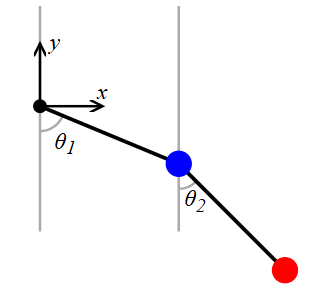
\includegraphics[width=0.3\textwidth]{primer_dveh_slika.png}
    \caption{Dvojno nihalo \cite{scipython:doublependulum}}
    \label{fig:dvojno_nihalo}
\end{figure}

Imamo dve žogici z masama $m_1$ in $m_2$ na palčkah dolžine $l_1$ in $l_2$ z zanemarljivo maso.

Recimo, da je prva žogica na $(x_1, y_1)$ in druga žogica na $(x_2, y_2)$. Te koordinate dobimo kot:
\begin{align*}
x_1 &= l_1 \sin(\theta_1), \\
x_2 &= l_1 \sin(\theta_1) + l_2 \sin(\theta_2), \\
y_1 &= -l_1 \cos(\theta_1), \\
y_2 &= -l_1 \cos(\theta_1) - l_2 \cos(\theta_2).
\end{align*}

\subsection*{Potencialna energija}

Potencialna energija je definirana kot $V = m g h$, kjer je višina žogice dana z $h = y$. \\
Za posamezni masi velja: $$h_1 = y_1, \quad h_2 = y_2.$$

Torej celotna potencialna energija sistema je:
\begin{align*}
V &= V_1 + V_2 \\
&= m_1 g(-l_1 \cos\theta_1) + m_2 g(-l_1 \cos\theta_1 - l_2 \cos\theta_2).
\end{align*}

\subsection*{Kinetična energija}

Kinetična energija vsake žogice je podana z izrazom $$T = \frac{1}{2} m v^2.$$

Hitrost žogic dobimo s pomočjo izraza $v = \sqrt{\dot{x}^2 + \dot{y}^2}$.

Odvodi koordinat so: \begin{align*}
\dot{x}_1 &= l_1 \dot{\theta}_1 \cos(\theta_1) \\
\dot{x}_2 &= l_1 \dot{\theta}_1 \cos(\theta_1) + l_2 \dot{\theta}_2 \cos(\theta_2) \\
\dot{y}_1 &= l_1 \dot{\theta}_1 \sin(\theta_1) \\
\dot{y}_2 &= l_1 \dot{\theta}_1 \sin(\theta_1) + l_2 \dot{\theta}_2 \sin(\theta_2)
\end{align*}

Skupna kinetična energija sistema je torej:
$$T = T_1 + T_2 = \frac{m_1}{2}(\dot{x}_1^2 + \dot{y}_1^2) + \frac{m_2}{2}(\dot{x}_2^2 + \dot{y}_2^2)$$

Lotimo se sedaj zapisa sistema Euler-Lagrangeevih enačb \cite{wikipedia:lagrangian} za $\mathcal{L} = T-V$:
\begin{align*}
    \mathcal{L} =& \, \frac{m_1}{2}(\dot{x}_1^2 + \dot{y}_1^2) + \frac{m_2}{2}(\dot{x}_2^2 + \dot{y}_2^2) + m_1 g(l_1 \cos\theta_1) + m_2 g(l_1 \cos\theta_1 + l_2 \cos\theta_2)\\
    =& \, \frac{m_1}{2}l_1^2 \dot{\theta_1}^2 + \frac{m_2}{2}(l_1^2 \dot{\theta_1^2} + l_2^2 \dot{\theta_2^2} + 2 l_1 \dot{\theta_1} l_2 \dot{\theta_2} \cos \theta_1 \cos \theta_2 + 2 l_1 \dot{\theta_1}l_2 \dot{\theta_2} \sin \theta_1 \sin \theta_2) \\
    &+ m_1 g l_1 \cos\theta_1 + m_2 g (l_1 \cos\theta_1 + l_2 \cos\theta_2)\\
    =& \, \frac{1}{2}m_1 l_1^2 \dot{\theta_1}^2 + \frac{1}{2}m_2(l_1^2 \dot{\theta_1}^2 + l_2^2 \dot{\theta_2}^2 + 2 l_1 l_2 \dot{\theta_1} \dot{\theta_2} \cos (\theta_1 - \theta_2)) + (m_1 + m_2)l_1 g \cos \theta_1 \\
    &+ m_2 l_2 g \cos \theta_2.
\end{align*}
Želimo dobiti enačbe oblike:
$$\frac{d}{dt} \Big(\frac{\partial \mathcal{L}}{\partial \dot{\theta_i}}\Big) = \frac{\partial \mathcal{L}}{\partial \theta_i}, \quad i = 1,2.$$
Najprej izpeljimo za $\theta_1$:
\begin{align*}
    \frac{\partial \mathcal{L}}{\partial \dot{\theta_1}} =& \, m_1 l_1^2 \dot{\theta_1} + m_2 l_1^2 \dot{\theta_1} + m_2 l_1 l_2 \dot{\theta_2} \cos(\theta_1 - \theta_2),\\
    \frac{d}{dt} \Big(\frac{\partial \mathcal{L}}{\partial \dot{\theta_1}}\Big) =& \, \, m_1 l_1^2 \ddot{\theta_1} + m_2 l_1 l_2 [\ddot{\theta_2} \cos(\theta_1 - \theta_2)- \dot{\theta_2} \sin(\theta_1 - \theta_2)(\dot{\theta_1}-\dot{\theta_2})]\\
    \frac{\partial \mathcal{L}}{\partial \theta_1} =& \, -m_2 l_1 l_2 \dot{\theta_1}\dot{\theta_2} \sin (\theta_1 - \theta_2) - (m_1 + m_2) l_1 g \sin\theta_1.
\end{align*}
Torej za $i=1$ dobimo:
\begin{align*}
    \frac{d}{dt} \Big(\frac{\partial \mathcal{L}}{\partial \dot{\theta_1}}\Big) - \frac{\partial \mathcal{L}}{\partial \theta_1} =& \, (m_1 + m_2) (l_1^2 \ddot{\theta_1}) + m_2 l_1 l_2 [\ddot{\theta_2}\cos (\theta_1 - \theta_2) + \dot{\theta_2}^2 \sin(\theta_1 - \theta_2)] \\
    &+(m_1 + m_2)l_1 g \sin \theta_1 = 0 \quad /:l_1.
\end{align*}
Podobno naredimo za $\theta_2$ in dobimo:
\begin{align*}
    \frac{\partial \mathcal{L}}{\partial \dot{\theta_2}} =& \, m_2 l_2^2 \dot{\theta_2} + m_2 l_1 l_2 \dot{\theta_1} \cos(\theta_1 - \theta_2)\\
    \frac{d}{dt} \Big(\frac{\partial \mathcal{L}}{\partial \dot{\theta_2}}\Big) =& \, m_2 l_2^2 \ddot{\theta_2} + m_2 l_1 l_2 [\ddot{\theta_1} \cos(\theta_1 - \theta_2) - \dot{\theta_1} \sin (\theta_1 - \theta_2)(\dot{\theta_1} - \dot{\theta_2})]\\
    \frac{\partial \mathcal{L}}{\partial \theta_2}=& \, -m_2 l_1 l_2 \dot{\theta_1} \dot{\theta_2} \sin(\theta_1 - \theta_2) - m_2 l_2 g \sin \theta_2
\end{align*}
Euler-Lagrangeeva enačba za $i=2$ se torej glasi:
\begin{align*}
    \frac{d}{dt} \Big(\frac{\partial \mathcal{L}}{\partial \dot{\theta_2}}\Big) - \frac{\partial \mathcal{L}}{\partial \theta_2} =& \, m_2 l_2^2 \ddot{\theta_2} + m_2 l_1 l_2 (\ddot{\theta_1} \cos(\theta_1 - \theta_2) - \dot{\theta_1}^2 \sin (\theta_1 - \theta_2)) + m_2l_2 g \sin \theta_2 =0 \quad /:l_2
\end{align*}

Dobimo sistem diferencialnih enačb:
\begin{align*}
    \theta_1: &\quad (m_1 + m_2)[l_1 \ddot{\theta_1} + g \sin \theta_1] + m_2 l_2 [\ddot{\theta_2} \cos(\theta_1 - \theta_2) + \dot{\theta_2}^2 \sin(\theta_1-\theta_2)] = 0\\
    \theta_2: &\quad m_2 [l_2 \ddot{\theta_2} + g \sin \theta_2] + m_2 l_1 [\ddot{\theta_1} \cos(\theta_1 - \theta_2) - \dot{\theta_1}^2 \sin(\theta_1 - \theta_2)] =0
\end{align*}

\section{Trojno nihalo}
Kaj pa bi se zgodilo, če vzamemo trojno nihalo? Predpostavimo, da na drugo žogico pripnemo preko vrvice $l_3$ še eno žogico z maso $m_3$.

Ta žogica je na položaju 
\begin{align*}
    x_3 &= l_1 \sin\theta_1 + l_2 \sin \theta_2 + l_3 \sin \theta_3\\
    y_3 &= - l_1 \cos \theta_1 - l_2 \cos \theta_2 - l_3 \cos \theta_3\\
    \dot{x_3} &= l_1 \dot{\theta_1} \cos \theta_2 + l_2 \dot{\theta_2} \cos \theta_2 + l_3 \dot{\theta_3} \cos \theta_3\\
    \dot{y_3} &= l_1 \dot{\theta_1} \sin \theta_2 + l_2 \dot{\theta_2} \sin \theta_2 + l_3 \dot{\theta_3} \sin \theta_3
\end{align*}

Za ta sistem imamo:
\begin{align*}
    V_3 =& \, m_1 g y_1 + m_2 g y_2 + m_3 g y_3 \\
    =& \, -(m_1 + m_2 + m_3)l_1 g \cos \theta_1 - \cos \theta_2 g l_2 (m_2 + m_3) - \cos\theta_3 l_3 m_3 g\\
    T_3 =& \, \frac{1}{2} m_1 (\dot{x_1}^2 + \dot{y_1}^2) + \frac{1}{2} m_2 (\dot{x_2}^2 + \dot{y_2}^2) + \frac{1}{2} m_3 (\dot{x_3}^2 + \dot{y_3}^2)\\
    =& \, \frac{1}{2} m_1 l_1^2 \dot{\theta_1}^2 + \frac{1}{2}m_2 [l_1^2 \dot{\theta_1}^2 + l_2 \dot{\theta_2}^2 + 2l_1l_2 \dot{\theta_1}\dot{\theta_2} \cos (\theta_1 - \theta_2)] + \frac{1}{2} m_3 [l_1^2 \dot{\theta_1}^2 + l_2 \dot{\theta_2}^2 \\
    &+ l_3^2 \dot{\theta_3}^2 + 2 l_1 l_2 \dot{\theta_1}\dot{\theta_2} \cos (\theta_1 - \theta_2) + 2 l_1 l_3 \dot{\theta_1}\dot{\theta_3} \cos (\theta_1 - \theta_3) + 2 l_2 l_3 \dot{\theta_2}\dot{\theta_3} \cos (\theta_2 - \theta_3)]\\
    \mathcal{L} =&\, T_3 - V_3
\end{align*}

Podobno kot za dvojno nihalo tudi tu dobimo sistem enačb za $\theta_i$, $i=1,2,3$. Če jih malo preuredimo, dobimo:
\begin{align*}
    \theta_1: &\quad (m_1 + m_2 + m_3) [l_1 \ddot{\theta_1} + g \sin \theta_1] + (m_2 + m_3) l_2 [\ddot{\theta_2} \cos (\theta_1 - \theta_2) + \dot{\theta_2}^2 \sin (\theta_1 - \theta_2)] \\
    & + m_3 l_3 [\ddot{\theta_3} \cos(\theta_1 - \theta_3) + \dot{\theta_3}^2 \sin (\theta_1 - \theta_3)]  = 0\\
    \theta_2: &\quad (m_2 + m_3) [l_2 \ddot{\theta_2} + g \sin \theta_2] + (m_2 + m_3) l_1 [\ddot{\theta_1} \cos (\theta_1 - \theta_2) - \dot{\theta_1}^2 \sin(\theta_1 - \theta_2)] \\
    & + m_3 l_3 [\ddot{\theta_3} \cos(\theta_2 - \theta_3) + \dot{\theta_3}^2 \sin(\theta_2 - \theta_3)] = 0\\
    \theta_3: &\quad m_3 [l_3 \ddot{\theta_3} - g \sin \theta_3] + m_3 l_1 [\ddot{\theta_1} \cos(\theta_1 -\theta_3) - \dot{\theta_1}^2 \sin (\theta_1 - \theta_3)] \\
    & + m_3 l_2 [\ddot{\theta_2}\cos(\theta_2 - \theta_3) - \dot{\theta_2}^2 \sin(\theta_2 - \theta_3)] = 0
\end{align*}

\textit{Zaenkrat sva dobili idejo za reukrzijo, ki izgleda nekako tako?:}
\begin{align*}
    \text{Za} \ \theta_1: &\quad (\sum_{i=1}^n m_i)[l_1 \ddot{\theta_1} + g \sin \theta_1] + \sum_{i=2}^n (\sum_{j=i}^n m_j) l_i (\ddot{\theta_i} \cos (\theta_1 - \theta_i) + \dot{\theta_i}^2 \sin(\theta_1 - \theta_i)) = 0\\
    \text{Za} \ \theta_n: &\quad m_n [l_n \ddot{\theta_n} + g \sin \theta_n] + m_n \sum_{i=1}^{n-1} l_i [\ddot{\theta_i} \cos(\theta_i - \theta_n) - \dot{\theta_i}^2 \sin (\theta_i - \theta_n)] = 0
\end{align*}

\printbibliography


\end{document}